\documentclass{article}
\usepackage{graphicx}
\usepackage{amsmath}
\usepackage{epsf}
\usepackage{xcolor}
\usepackage{float}
\newtheorem{theorem}{Theorem}
\setlength{\topmargin}{0.1in}
\setlength{\oddsidemargin}{0in}
\setlength{\evensidemargin}{0in}
\setlength{\headheight}{0in}
\setlength{\headsep}{0in}
\setlength{\textheight}{9in}
\setlength{\textwidth}{6.5in}
% require that floats fill 90% of a page in order for that page to be
% ``float-only''
\renewcommand{\dblfloatpagefraction}{0.9}
\renewcommand{\floatpagefraction}{0.9}
\newenvironment{bibparagraph}{\begin{list}{}{ %
    \setlength{\labelsep}{-\leftmargin} %
    \setlength{\labelwidth}{0pt} %
    \setlength{\itemindent}{-\leftmargin} %
    \setlength{\listparindent}{0pt}}}{\end{list}}
\def\makefigure#1#2{\begin{figure}
\begin{center}
\input{#1}
\end{center}
\caption{#2}
\label{#1}
\end{figure}}

\def\limplies{\; \supset \;}
\def\land{\: \wedge \:}
\def\lor{\: \vee \:}
\def\iff{\; \equiv \;}
\def\lnot{\neg}
\def\lforall#1{\forall \: #1 \;}
\def\lexists#1{\exists \: #1 \;}
\def\glitch#1{{\tt #1}} % glitch on
%\def\glitch#1{} % glitch off
\def\comment#1{}
\def\pnil{[\;]}
\def\pif{\; \mbox{\tt :- } \;}
\def\tuple#1{$\langle #1\rangle$}
\def\mtuple#1{\langle #1\rangle}
\def\ceiling#1{\lceil #1\rceil}
\def\floor#1{\lfloor #1\rfloor}
\def\centerps#1{\begin{center}
\leavevmode
\epsfbox{#1}
\end{center}}
\def\argmax{\mathop{\rm argmax}}
\def\argmin{\mathop{\rm argmin}}
\def\grad{\nabla\!}
\def\celsius{^\circ\mbox{C}}
%\long\def\answer#1{}  % comment out for solutions
%\long\def\question#1{#1} % comment out for solutions
\long\def\answer#1{{\color{blue}{\sl #1}}}  % comment in for solution
\long\def\question#1{} % comment in for solution
%\renewcommand{\labelenumi}{(\alph{enumi})}

\def\x{{\bf x}}
\def\w{{\bf w}}

\begin{document}
{\Large
\begin{center}
AI534 --- Written Assignment 4 ---
\end{center}
}
%Please submit electronically via TEACH in a single pdf file.
\begin{enumerate}
\item (6 pts) Consider the following decision tree:\\
%{\epsfxsize=5in
%\centerps{tree1.eps}
%}
\begin{figure}[h]
\begin{center}
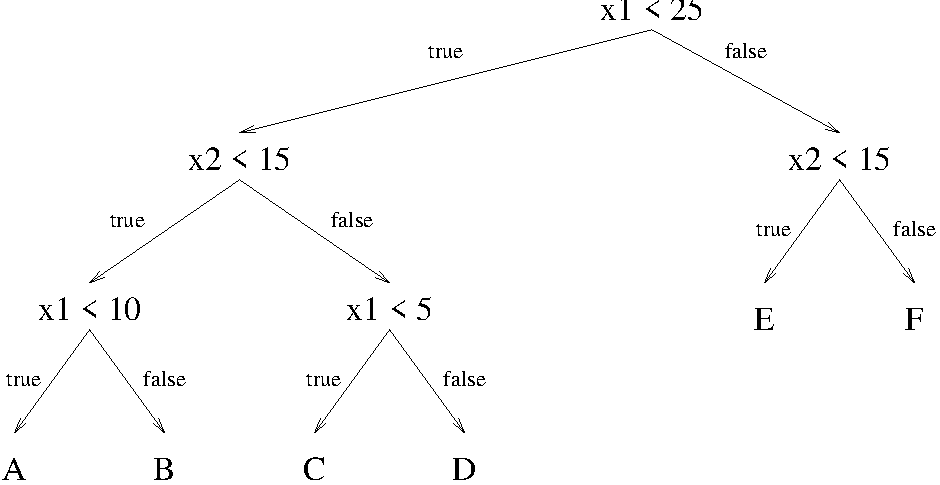
\includegraphics[width=4in]{tree1.pdf}
\end{center}
\end{figure}

\begin{enumerate}

\item (2 pts) Draw the decision boundaries defined by this tree. Each
leaf of the tree is labeled with a letter.  Write this
letter in the corresponding region of input space.\\

\answer{Your answer here
First, let us name the regions divided the boundaries as follows
\begin{center}
    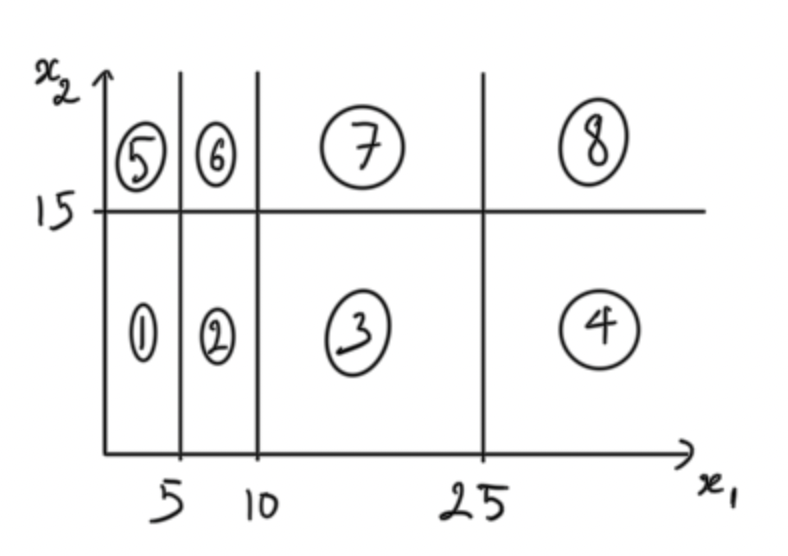
\includegraphics[scale=0.5]{q1a.png}    
\end{center}
}

The areas covered by the letters are: \newline
A: 1 + 2 \newline
B: 3 + 4 \newline
C: 5 \newline
D: 6 + 7 + 8 \newline
E: 4 \newline
F: 8 \newline

\item (2 pts) Give another decision tree that is syntactically
different but defines the same decision boundaries.  This
demonstrates that the space of decision trees is
syntactically redundant.  \\

\answer{
Your answer here} 

\item (2 pts) How does this redundancy influence learning (does it make it easier or harder to find an accurate tree)?\\
\answer{Your answer here
}

\end{enumerate}
\item (6 pts) In the basic decision tree algorithm (assuming we always create binary splits), we choose the feature/value pair with the maximum information gain as the test to use at each internal node of the decision tree.  Suppose we modified the algorithm to choose at random from among those feature/value combinations that had non-zero mutual information, and we kept all other parts of the algorithm unchanged.

\begin{enumerate}
\item (2 pts) What is the maximum number of leaf nodes that such a
decision tree could contain if it were trained on $m$ (distinct)
training examples?

\answer{Your answer here}

\item (2 pts) What is the maximum number of leaf nodes that a decision
tree could contain if it were trained on $m$ training
examples using the original maximum mutual information
version of the algorithm?  Is it bigger, smaller, or the
same as your answer to (b)?

\answer{Your answer here}

\item (2 pts)How do you think this change (using random splits vs. maximum information mutual information splits) would affect the accuracy of the decision trees produced on average?  Why?

\answer{Your answer here
}

\end{enumerate}
\item (8 pts) Consider the following training set:

\begin{center}
\begin{tabular}{|c|c|c|c|}\hline
A&B&C&Y\\ \hline
0&1&1&0 \\ \hline
1&1&1&0 \\ \hline
0&0&0&0 \\ \hline
1&1&0&1 \\ \hline
0&1&0&1 \\ \hline
1&0&1&1 \\ \hline
\end{tabular}
\end{center}

Learn a decision tree from the training set shown above using the information gain criterion. Show your steps, including the calculation of information gain (you can skip $H(y)$ and just compute $H(y|\x)$) of different candidate tests. You can randomly break ties (or better, choose the one that give you smaller tree if you do a bit look ahead for this problem).

\answer{Your answer here}

\item (5 pts) Please show that in iteration $l$ of Adaboost, the weighted error of $h_l$ on the updated weights $D_{l+1}$ is exactly 50\%. In other words, $\sum_{i=1}^N D_{l+1}(i) I(h_l(X_i)\neq y_i) = 50\%$, where $I(\cdot)$ is the indicator function that takes value 1 if the argument is true. (Hint: start with the condition that, post update, the total weight of correct examples equals the total weight of in-correct examples, i.e., 50\% each.)

\answer{Your answer here
}

\item {\bf HAC}. (4pts) Create by hand the clustering dendrogram for the following samples of ten points in one dimension.
\[Sample=( - 2.2, -2.0, -0.3, 0.1, 0.2, 0.4, 1.6, 1.7, 1.9, 2.0)\]
\begin{itemize}
\item[a.] (2pts) Using single link.\\
\answer{Your solution here
}

\item[b.] (2pts) Using complete link \\
\answer{Your solution here
}

\end{itemize}


\item (6 pts)Deriving Kmeans for $L_1$ norm. 
Consider replacing the distance function used for Kmeans with $L_1$ norm with the following objective:
\[\min_{\mu_1,...,\mu_K,C_1,...,C_K}\sum_{i=1}^K \sum_{x\in C_i} |x-\mu_i|\]

\begin{itemize}
    \item (3 pts) Show that given fixed cluster assignment $C_1, ..., C_K$, the prototype $\mu_i$ that optimizes the above objective can be obtained by taking element-wise median of all the points in cluster $i$.

    \answer{Your answer here
    }

\item  (3 pts) Modify the kmeans algorithm for this $L_1$ based objective.\\
\answer{ Your answer goes here.}
\end{itemize}
\end{enumerate}
\end{document}
